\section{ВЕКТОРЫ НА ПЛОСКОСТИ}

\textbf{2322.} Вектор $\overrightarrow{AB}$ $-$ это направленный отрезок, точки $A(x_A, y_A)$ и $B(x_B, y_B)$ являются его началом и концом. Первая координата называется абсциссой, вторая $-$ ординатой. Координаты вектора $-$ это разности координат его конца и начала. Поэтому для вектора принято обозначение:
\[
\overrightarrow{AB}(x_B-x_A, y_B-y_A).
\]
В нашем случае: $x_B-x_A=-6, \; x_A-6=3-6=-3.$ \newline \null \hspace*{\fill} Ответ: $-$3.

\textbf{2323.} $y_B-y_A=2, \; y_B=y_A+2=2+2=4.$ \newline \null \hspace*{\fill} Ответ: 4.

\textbf{2324-2326} $-$ аналогичные задачи.

\textbf{2327.} $x_B-x_A=8, \;x_B=x_A+8=12+8=20$. Аналогично $y_B-y_A=-3, \; y_B=y_A-3=-1-3=-4.$ Таким образом, $x_B+y_B=20-4=16.$ \newline \null \hspace*{\fill} Ответ: 16.

\textbf{2328-2331} $-$ аналогичные задачи.

\textbf{2332.} $y_B-y_A=3, \; y_A=y_B-3=1-3=-2.$ \newline \null \hspace*{\fill} Ответ: $-$2.

\textbf{2333-2341} $-$ аналогичные задачи.

\textbf{2342.}

{\centering 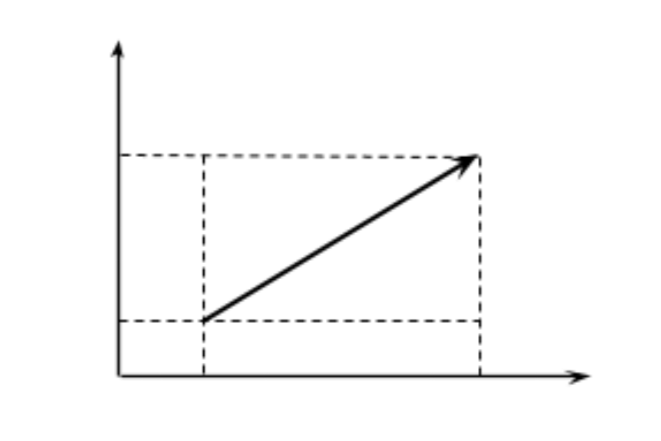
\includegraphics[width=0.5\linewidth]{Geometry/Content/54.png}
	
}

На рисунке изображена прямоугольная система координат и вектор $\overrightarrow{AB}(x_B-x_A, y_B-y_A)$. на плоскости. Длину вектора  можно найти по теореме Пифагора:
\[
AB=|\overrightarrow{AB}|=\sqrt{(x_B-x_A)^2+(y_B-y_A)^2}.
\]
Это неотрицательное число, равное длине отрезка $AB$. Если концы вектора совпадают,  и он стягивается в точку, такой вектор называется нулевым; его длина равна нулю, а направление не имеет смысла. В остальных случаях длина вектора положительна.

В нашем случае $a = |\vec{a}|=\sqrt{(-12)^2+(-9)^2}=\sqrt{144+81}=15.$ \newline \null \hspace*{\fill} Ответ: 15.

\textbf{2343-2346} $-$ аналогичные задачи.

\textbf{2347.} В данном случае вектор $\overrightarrow{AC}$ построен на диагонали параллелограмма $ABCD$ и его длина равна длине диагонали:
\[
AC=|\overrightarrow{AC}|=\sqrt{28^2+21^2}=35.
\]\null \hspace*{\fill} Ответ: 35.

\textbf{2348-2351} $-$ аналогичные задачи.

\textbf{2352.} Если система координат на плоскости выбрана, то две простейшие операции над векторами выполняются с помощью соответствующих операций над их координатами, а именно:

a) произведением вектора $\vec{a}(a_x, a_y)$ на число $\lambda$ называется вектор $\lambda \cdot = (\lambda a_x, \lambda a_y)$; его координаты получаются умножением на число $\lambda$ соответствующих координат вектора $\vec{a}$;

б) суммой векторов $\vec{a}(a_x, a_y)$ и $\vec{b}(b_x, b_y)$ называется вектор $\vec{c}=\linebreak=\vec{a}+\vec{b}=(a_x+b_x, a_y+b_y)$; координаты этого вектора равны суммам соответствующих координат векторов $\vec{a}$ и $\vec{b}$. 

В данной задаче удобно выбрать прямоугольную систему координат естественным образом: начало координат совместить с вершиной $A$ прямоугольника, а оси координат направить вдоль его смежных сторон $AD$ и $AB$.

{\centering 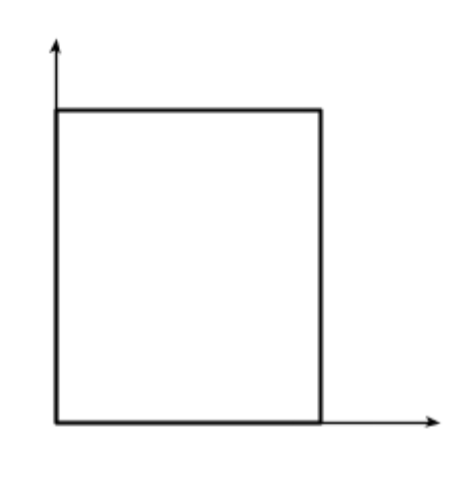
\includegraphics[width=0.4\linewidth]{Geometry/Content/55.png}
	
}

В такой системе  координаты векторов $\overrightarrow{AB}$ и $\overrightarrow{AD}$ записываются очень просто: $\overrightarrow{AB} = (32, 0)$, $\overrightarrow{AD} = (0, 24)$. Тогда $\overrightarrow{AB} + \overrightarrow{AD} = \linebreak =(32, 24)$, а длина этого вектора равна $|\overrightarrow{AB} + \overrightarrow{AD}| = \sqrt{32^2+24^2}=\linebreak=40.$ \newline \null \hspace*{\fill} Ответ: 40.

\textbf{Замечание.} В этой простой задаче можно сразу сказать: сумма двух векторов $-$ это вектор, построенный на  диагонали параллелограмма (в данном случае $-$ прямоугольника), и сразу вычислить длину этой диагонали. 

\textbf{2353-2356} $-$ аналогичные задачи.

\textbf{2357.}  Используем систему координат задачи \textbf{2252}. Тогда, очевидно
$\overrightarrow{AB}=(16, 0)$, $\overrightarrow{AD} = (0, 30)$, $\overrightarrow{AB} - \overrightarrow{AD} = (16, -30)$, так что $|\overrightarrow{AB} - \overrightarrow{AD}|=\sqrt{16^2+(-30)^2}=34$. \newline \null \hspace*{\fill} Ответ: 34.

\textbf{2358-2361} $-$ аналогичные задачи.

\textbf{2362.} Еще более ярким примером продуктивности координатного подхода являются задачи, связанные со скалярным произведением векторов. Геометрическая трактовка: скалярное произведение векторов $\overrightarrow{a}$ и $\overrightarrow{b}$ $-$ это число, равное произведению длин векторов на косинус угла $\phi$ между ними:
\[
\vec{a}\cdot \vec{b}=\vec{a}\;
\vec{b}=|\vec{a}|\cdot|\vec{b}|\cdot\cos{\phi}\]

Координатная трактовка: скалярное произведение векторов \linebreak $\vec{a}(a_x, a_y)$ и $\vec{b}(b_x, b_y)$ есть число $\vec{a}\cdot \vec{b}=\vec{a}\;
\vec{b} = a_xb_x+a_yb_y$. Ни длины векторов, ни угол между ними не нужны: все расчеты ведутся с их координатами.

Конечно, если заданы длины векторов и угол между ними, следует воспользоваться геометрическим определением скалярного произведения. Например, в данной задаче совершенно очевидно, что векторы $\overrightarrow{AB}$ и $\overrightarrow{AD}$ перпендикулярны, $\cos{90^\circ}=0$, так что длины сторон и не нужны, ясно, что $\overrightarrow{AB}\cdot\overrightarrow{AD}=0$ \newline \null \hspace*{\fill} Ответ: 0.                       

Но такого рода задачи скорее являются исключением, чем правилом. Хотя мои предпочтения скорее связаны не со школьными задачами, а со студенческими.

\textbf{2363-2366} $-$ аналогичные задачи, все они банально просто решаются с помощью геометрического подхода. В ответах одни нули, т.к. векторы перпендикулярны и их длины не имеют значения.

\textbf{2367.}

{\centering 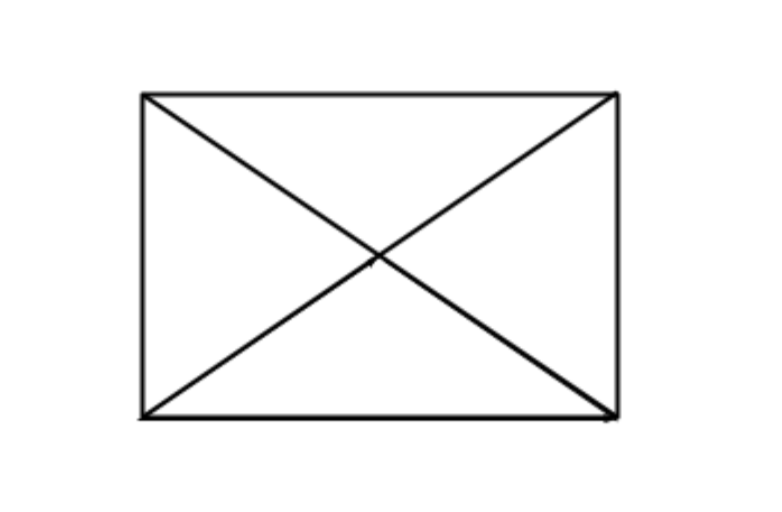
\includegraphics[width=0.5\linewidth]{Geometry/Content/56.png}
	
}

Геометрически векторы можно складывать по правилу цепочки. Если требуется сложить несколько векторов, то второй пристраивают к концу первого, третий $-$ к концу второго, и т.д. Суммой таких векторов, выстроенных цепочкой, является замыкающий цепочку вектор, проведенный из начала первого вектора в конец последнего. 

Следует также отметить, что в математике вектор свободный или плавающий, т.е. его можно произвольно перемещать параллельно самому себе. Поэтому в нашем случае $\overrightarrow{BO}=\overrightarrow{OD}$, а по правилу цепочки $\overrightarrow{AO}+\overrightarrow{OD}=\overrightarrow{AD}$. Поэтому $|\overrightarrow{AO}+\overrightarrow{OD}|=|\overrightarrow{AD}|=$\newline$=AD=68.$ \newline \null \hspace*{\fill} Ответ: 68.

\textbf{2368-2371} $-$ аналогичные задачи. 

\textbf{2372.} Если поменять местами начало и конец какого-либо вектора, то $\overrightarrow{MN}=-\overrightarrow{NM}$. В нашем случае (см. чертеж к задаче \textbf{2367}): $\overrightarrow{AO} - \overrightarrow{BO} = \overrightarrow{AO} + \overrightarrow{OB} = \overrightarrow{AB}$, так что $|\overrightarrow{AO}+\overrightarrow{OB}|=|\overrightarrow{AB}|=\linebreak=AB=33.$ \newline \null \hspace*{\fill} Ответ: 33.

\textbf{2373-2376} $-$ аналогичные задачи.

\textbf{2377.}

{\centering 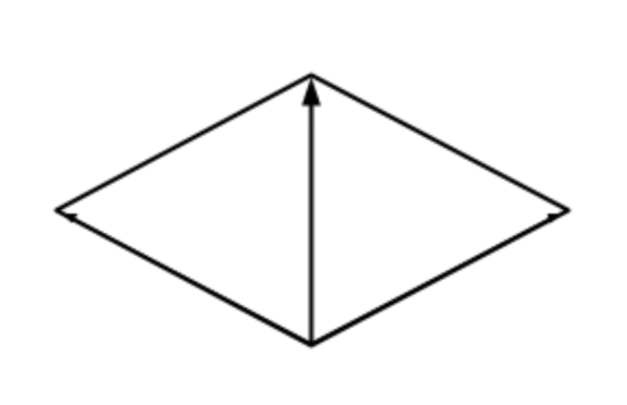
\includegraphics[width=0.5\linewidth]{Geometry/Content/57.png}
	
}
\[
\overrightarrow{AB}+\overrightarrow{AD}=\overrightarrow{AC}, \; |\overrightarrow{AB} + \overrightarrow{AD}| = |\overrightarrow{AC}|=AC=33.
\] \newline \null \hspace*{\fill} Ответ: 33.

\textbf{2378-2381} $-$ аналогичные задачи.

\textbf{2382}. См. чертеж задачи \textbf{2377}. $\overrightarrow{AB} - \overrightarrow{AD}=\overrightarrow{DA}+\overrightarrow{AB}=\overrightarrow{DB},$ $|\overrightarrow{AB}-\overrightarrow{AD}|=|\overrightarrow{DB}|=DB=67.$ \newline \null \hspace*{\fill} Ответ: 67.  

\textbf{2383-2386} $-$ аналогичные задачи.

\textbf{2387.}

{\centering 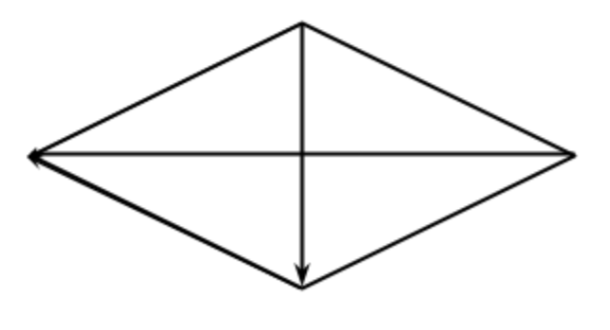
\includegraphics[width=0.5\linewidth]{Geometry/Content/58.png}
	
}

Диагонали ромба взаимно перпендикулярны и в точке пересечения делятся пополам. Поэтому $CO=\frac{24}{2}=12$, $BO=\frac{45}{2}=22,5$, а $|\overrightarrow{AB}=\overrightarrow{AC}|=|\overrightarrow{CA}-\overrightarrow{AB}|=\overrightarrow{CB}=CB=\sqrt{CO^2+BO^2}=\linebreak=\sqrt{12^2+(22,5)^2}=25,5.$ \newline \null \hspace*{\fill} Ответ: 25,5.

\textbf{2388-2391} $-$ аналогичные задачи.

\textbf{2392.}  См. чертеж задачи  \textbf{2387}. $|\overrightarrow{AO}+\overrightarrow{BO}|=|\overrightarrow{AO}+\overrightarrow{OD}|=\overrightarrow{AD}=\linebreak=AD=\sqrt{AO^2+DO^2}=\sqrt{\left( \frac{3}{2} \right)^2 + \left( \frac{4}{2} \right)^2}=2,5.$ 

\textbf{2393-2401} $-$ аналогичные задачи.

В задачах \textbf{2402-2406} все пары векторов перпендикулярны (см. чертеж \textbf{2387}), поэтому их скалярные произведения равны нулю.

\textbf{2407.}

{\centering 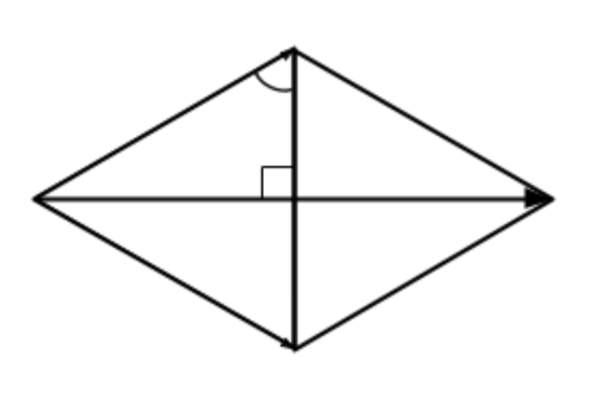
\includegraphics[width=0.5\linewidth]{Geometry/Content/59.png}
	
}

Пусть $ABCD$ $-$ ромб с острым углом $\angle BAC = 60^\circ$. Проведем его диагонали, пересекающиеся в точке $O$. В силу симметрии $\Delta ABC$ $-$ равносторонний и по условию задачи его сторона $AB=47\sqrt{3}$. Из геометрических соображений $\overrightarrow{AB}+\overrightarrow{AC}=\overrightarrow{AD}$
и нам требуется вычислить длину диагонали ромба $AD$. Очевидно
\[
AD=2AO=2AB\sin{60^\circ}=2\cdot47\sqrt{3}\cdot\frac{\sqrt{3}}{2}=141.
\]  \newline \null \hspace*{\fill} Ответ: 141. 

\textbf{2408-2411} $-$ аналогичные задачи.

\textbf{2412.} Из чертежа задачи \textbf{2407} следует, что $\overrightarrow{AB}=\overrightarrow{CD}$, $-\overrightarrow{AC}=\linebreak=\overrightarrow{CA} = \overrightarrow{DB}$, поэтому $\overrightarrow{AB}-\overrightarrow{AC}=\overrightarrow{CD}+\overrightarrow{DB}=\overrightarrow{CB}$, а $|\overrightarrow{CB}|=\linebreak=CB=AB=42$. \newline \null \hspace*{\fill} Ответ: 42.
 
\textbf{2413-2416} $-$ аналогичные задачи.

\textbf{2417.}  Угол между сторонами правильного треугольника равен $60^\circ$, поэтому скалярное произведение равно $4\cdot40\cdot\cos{60^\circ}=800$. \newline \null \hspace*{\fill} Ответ: 800.

\textbf{2418-2421} $-$ аналогичные задачи.
